\documentclass{csfourzero}
\usepackage{url, natbib, upquote, multicol, caption, subcaption, float}

\title{The effect of corruption on search engine query prediction}
\author{Charlie F.\ Egan}
\date{\today}

\bibliographystyle{plain}
\abstract{Search engines have are able to learn from user behavoir to improve their results. Rather than relying on a traditional spelling correction algorithms, user query patterns can be used to train the system and provide more accurate predictions. This report investigates how increasingly corrupted input effects the prediction accuracy of the system and well as how each in a number of top search engines compare in their ability to predict intended input. Related work and concepts are also discussed. It was found that search engines differ significantly in their prediction accuracy and that there is no relation between the word length performance.}

\begin{document}
\maketitle

\section{Introduction}
\label{sec:intro}

Search engines offering query predictions are the research interest of the project. Search engines offer predictions to overcome corruption in user queries, where corruption is the combined effect of one or more typographical errors. While prediction performance is high, the details of processes behind predictions are not always fully disclosed. Failed user queries followed by a user's own corrections can build an aggregated list of corrupted inputs for an intended result, for longer queries the probabilities for words in context can also be accounted for \cite{noampatent}. Probabilistic edit-distance implementations are also used \cite{howtospellcorrector}.

The project aim is to evaluate the variation in the prediction accuracy in responses, for increasingly corrupted terms, queried on a number of common search engines. Prediction accuracy is capability of a search engine suggest or adopt the intended term, given a corrupted version. The effect of query length in characters, for a given rate of corruption, is also investigated as part of the project.

Information about search engine prediction accuracy, would be useful for those making mechanical use of search engines. A ranked list of search engines by prediction accuracy could also be of interest to those with poor spelling or dexterity from conditions such as Dyslexia or Parkinson's disease. More generally, the relationship between corruption rates and query lengths for information transfer using an error prone or noisy channel is of broader interest.

Sections 2-7 cover: spelling correction background as a task in natural language processing, the research questions, the design of the comparison experiments, the results, their discussion and conclusion respectively.

\section{Background and Related Work}
\label{sec:lit}

``Correction is the task of substituting the well-spelled hypotheses for misspellings." \cite{webuser4google2009}

Computerized spelling correction has been undergoing research since 1957 \cite{jameslpeterson1980beginning}. Early approaches offered predications for strings with typographical errors by calculating edit distance \cite{1992correctiondiscussion}. The edit distance of two strings is the number of edit operations required to transform one string into another \cite{introIR}. In 1966 Levenshtein described a model for such transformations \cite{levenshtein1966binary}. \textit{Levenshtein distance} has been the basis for many error models used in spelling correction implementations since.

However, calculating edit distances for a string against large dictionaries is computationally expensive \cite{2009adaptivespellchecker}. A number of more recent implementations have been built using a \textit{Noisy Channel Model}, based on Shannon's \textit{Noisy Channel Theorem}.

One such program, \textit{correct}, detailed in a paper by Kernighan et al. (1990), offered correction from non-word errors detected by the Unix \textit{spell} program \cite{originalnoisychannel}. The tool generated all candidate corrections for a misspelling by applying a single deletion, insertion, transposition or substitution at each position. These candidate corrections are ranked by a combination of their frequency in a large corpus and the probability of the misspelling given the correction. The later probability, and the model of the noisy channel, is calculated using 'confusion matrices' that store the relative frequencies of different single letter corruptions for pairs of letters. This error model was extended by Brill \& Moore (2000) \cite{betternoisychannel} to represent 'string to string' edits for words with multiple errors. This improvement led to a 52\% reduction in spelling correction errors.

Corruptions of search terms over a noisy channel is comparable to the study of single nucleotide polymorphisms and copy-number variations in Genetics, deep space telecommunications and wireless video streaming.

Search engine query correction poses new challenges. 10-15\% of search engine queries contain errors, and short queries make contextual approaches used in word processing impractical \cite{webuserpoweredspelling}. Corrections for non-word, typographical errors cannot be not fully accounted for with dictionaries \cite{webuser3}, for example, \textit{verizon} may be the intended term but would likely be corrected to \textit{version} or \textit{horizon} with a traditional approach. Real word (cognitive) errors, such as \textit{'an introduction to \textbf{sea} programming'}, are also hard to model in dictionary implementations.

The first documented approach to make use of user search patterns was that of Brill \& Cucerzan in 2004 \cite{webuserpoweredspelling}. Their implementation compared search engine query logs  with a large corpus to gather candidate corrections and used a context-dependent, weighted, edit distance error model was used to make comparisons. Given that the majority of queries are correct, the transformations can be iteratively applied to arrive at more common (correct) queries. The results of the system, the first published approached to utilize query logs, aligned 82\% of the time with human annotators with high precision and recall statistics. This approach was improved upon with the inclusion of additional metrics such as page count (for a given term) by Chen et al. (2007) \cite{webuser3}.

A similar approach employed an \textit{Expectation Maximization algorithm} instead of a of corpus of corrections \cite{webuser2learningerrormodel}, while comparable, it did not perform as well as implementations that relied on manually derived informations. A corpus and language independent implementation first appeared in 2009, Whitelaw et al.\cite{webuser4google2009}. This was the first system to remove the hand-labeled data requirement. Information about misspellings are inferred from their use in query logs, common queries are used as a list of candidate corrections. The system is built fundamentally on the Noisy Channel Model \cite{claudeshannon1948}.

Despite top search companies contributing much to the area \cite{microranker, webuser3, webuserpoweredspelling, microranker, microphone, webuser4google2009}, comparable information about their implementations is not available. Additionally, the effect of data size on error correction rates over a error prone channel does not appear to have been made.

\section{Research question}
\label{sec:rq}

While spelling correction automation is an active topic of research, little is known of the implementations used by search engine companies. An aim of this project is to superficially investigate these systems and learn whether or not their implementations differ. The research questions for the project are as follows:

\begin{itemize}
  \item{What is the effect of query length on the suggestion accuracy for a given rate of corruption?}
  \item{Is there a significant difference in prediction accuracy between search engines?}
\end{itemize}

To address these questions the prediction accuracy for a number of search engines will be compared when queried with corrupted terms of various lengths. Each search engine will be tested with the same set of corrupted terms and the accuracy of their returned predictions recorded.

The following search engines will be tested: \textit{Ask, Baidu, Bing, DuckDuckGo, Google, Sogou, Yahoo, Yandex and Youdao}. These non-aggregating search engines all offer suggestions for misspelled queries and represent a majority of global general search engines \cite{searchenginewiki}. A parallel scraper has been implemented to collect the results of each for a given query \cite{scraper}. Five instances of this scraper will be deployed to disposable environments on the Heroku PaaS and requests made against instance to gather results from a local script.

The seed terms selected to derive corruptions will be website brands of a given length. Brands that are either four, eight or twelve characters in length were selected to allow a constant corruption rate of 25\% to be applied. Longer word seeds were few and were excluded to ensure predominantly single word brands were used. Seed terms are listed in Appendix 1, their selection is detailed in the following section.

Corruptions will be generated from seed terms using a substitution algorithm, see Appendix 2. A corruption is applied by selecting a random, unchanged character and substituting it with an adjacent key on the keyboard to simulate typographical (non-word) errors. Transformations, as based on the US (UK Macintosh) keyboard, are listed in Appendix 3. Insertions of additional letters, letter deletions and transpositions will are not included as part of this study.

In this experiment all queries are of single class, single word queries and search engines will be compared on their Accuracy alone. That is, for a given query set, the percentage of corrupted queries that cause the search engine to return the seed term as a correction. Given their rarity, collisions of corrupted spellings with other uncorrupted queries assumed to be insignificant.

\section{Experimental Design}
\label{sec:exp}

The null hypotheses for the experiment are as follows:
\begin{itemize}
  \item{At a constant rate of corruption, accuracy is not significantly affected by the query length in characters. (\textbf{H1})}
  \item{Search engines do not differ significantly in their average accuracy for a range of query lengths. (\textbf{H2})}
\end{itemize}

The target population is all user search queries that are the result of one or more typographical errors. Due to search engine rate-limiting and time constraints it is infeasible to test these in large numbers. Random seed terms such as strings of words would not be representative of real world queries and have poor rankings. A consistent collection of realistic query phrases is challenging to generate without introducing bias. In this experiment Alexa ranked word (or compound word) terms 4, 8 and 12 characters in length were selected from the Top 500 list \cite{alexatop500}. These are highly representative of typical queries and can be consistently corrupted at 25\%, such restrictions help reduce bias that query selection might introduce. There were too few 16 character terms for them to be included as an additional set of seed terms. Only .com brands were selected to avoid queries for the same brand on multiple top-level domains, this could introduce bias and is a weakness of the study.

At each query length (4, 8, 12), 100 terms were generated from the seeds with constant 25\% corruption using the algorithm in (Appendix 2). See Appendix 1 for seed terms used for each length. Accuracy is defined as the percentage of seed terms returned for their corresponding corrupted term. The search engine accuracy and term length are the independent and dependent variables respectively.

To test the hypotheses, the search engine responses for the each of the 100 corrupted terms for each length will be recorded. The accuracies of each search engine at each word length will be compared. Should the differences in average accuracy be found to be significant (p \textless 0.05) between length then there will be reason to reject the null hypothesis \textbf{H1}.

If the search engine accuracy difference is found to be significant (p \textless 0.05) then this will be cause to reject \textbf{H2}.

\section{Results}
\label{sec:results}

Present the results. A good way to organize this is via subsections
for each hypothesis you tested. Include graphs of results
, tests of significance, etc.

Guide length: 500 words.

The results suggest that all decreased in accuracy as the number of corruptions increased. Also x did better then y - quote values to support / highlight things in the table

Then do a section for each comparison and hypothesis / question 5.1 5.2 - say was was and was not significant, in response to the question. Quote those p values!

Quote the p values and the difference in the results from the tukey HSD

\begin{figure}
  \centering
  \begin{minipage}{.5\textwidth}
    \centering
    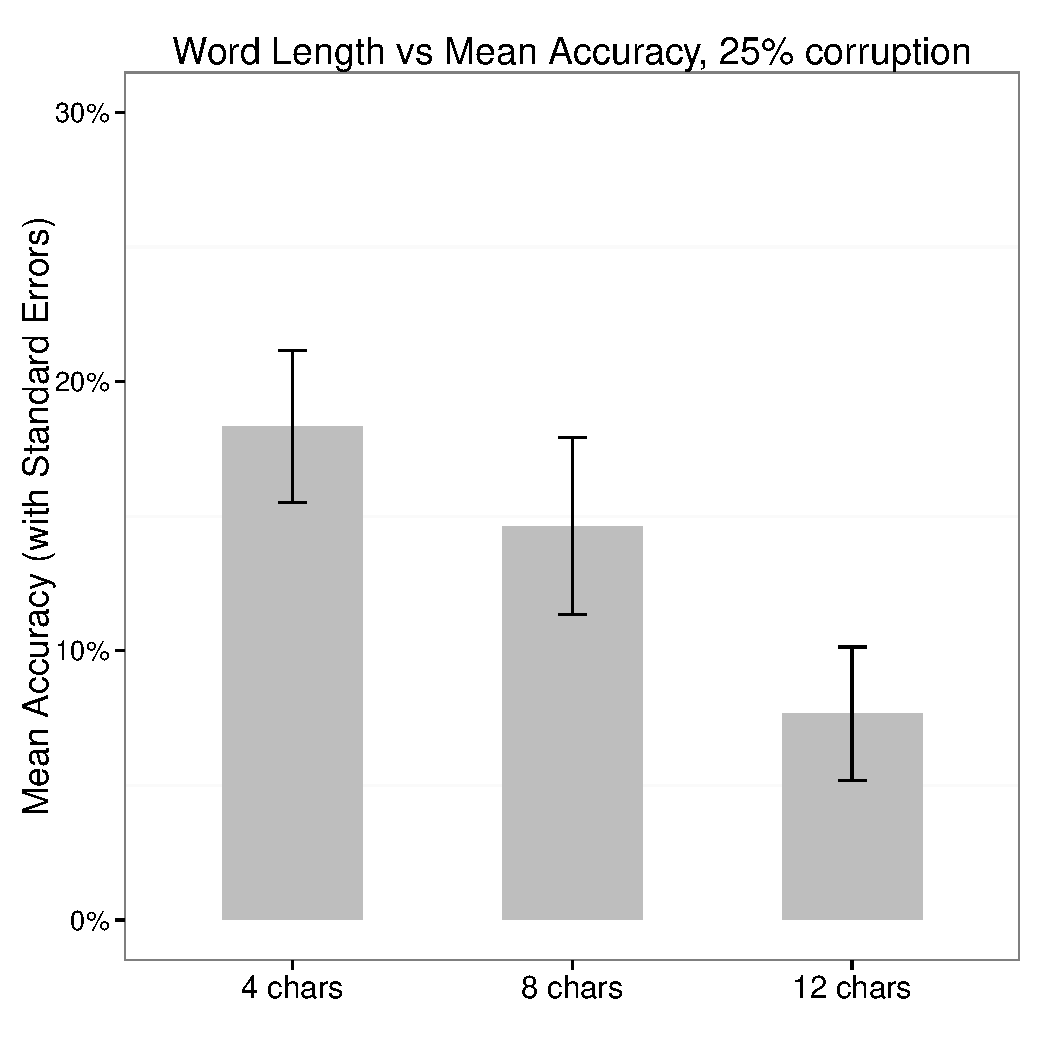
\includegraphics[width=\textwidth]{len_vs_acc}
    \captionof{figure}{Mean search engine accuracy for each query length}
    \label{fig:lengths}
  \end{minipage}%
  \begin{minipage}{.5\textwidth}
    \centering
    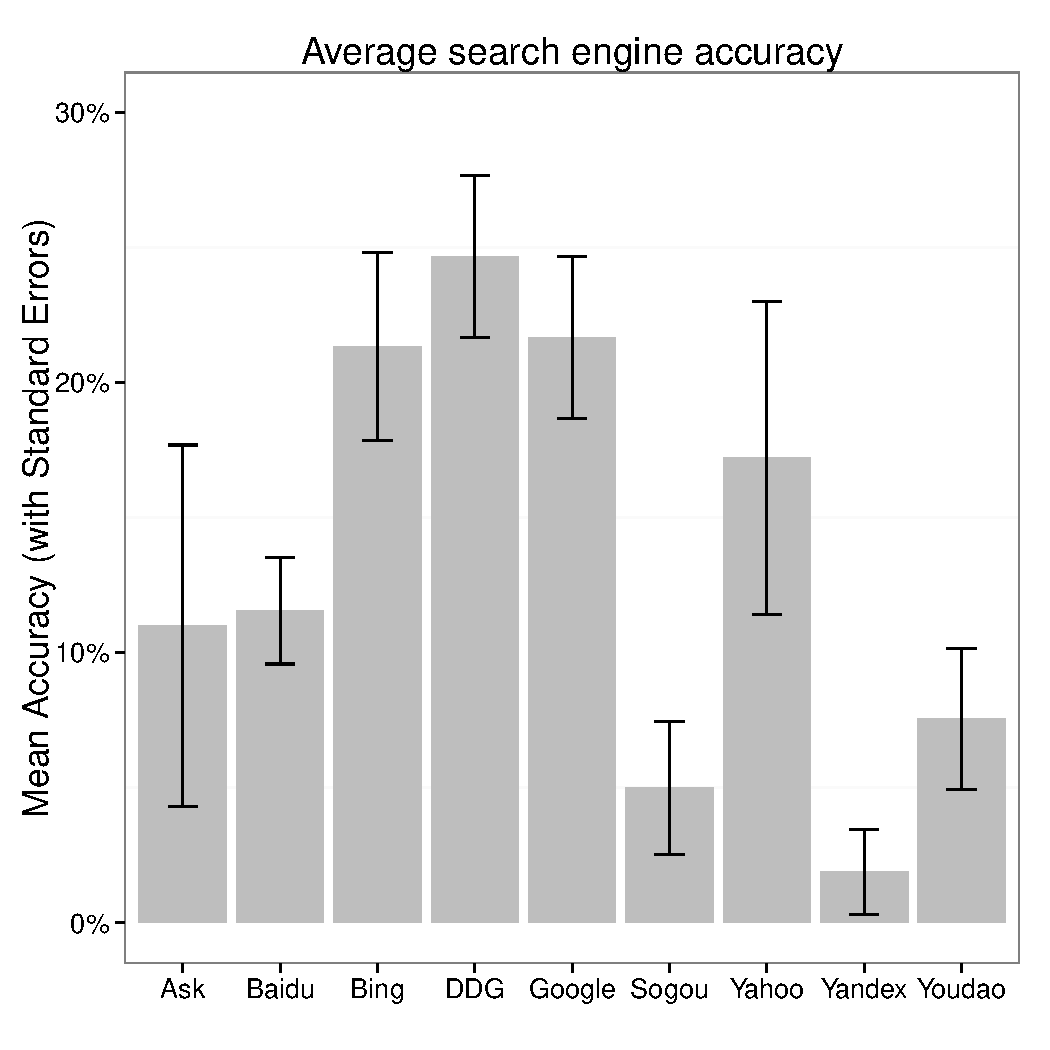
\includegraphics[width=\textwidth]{eng_vs_acc}
    \captionof{figure}{Mean accuracies over all query lengths}
    \label{fig:searchengines}
  \end{minipage}
\end{figure}

Figure~\ref{fig:lengths} shows the average for all nine search engines for each query length. Figure~\ref{fig:searchengines} shows the average accuracy over all query length for each search engine. Error bars in both figures represent standard errors in the mean values.

The results suggest that correction accuracy decreases as the query length increases. The effect is most apparent for 12 character queries. While queries 4 and 8 characters in length have more similar accuracy values there still appears to be a difference. The results also show a clear difference in search engine correction accuracy performance. Surprisingly, DuckDuckGo returned the most accurate predictions, performing 11\% above average and 23\% above Yandex, the poorest performing engine. DuckDuckGo is the search engine with the second lowest Alexa rank of those under test. Also of note was the difference between 4 and 8 characters for Google - it was the only search engine to perform better on 8 character queries.

\subsection{Term length comparison}
An f-test was performed for the results of all search engines at the each of the 3 query lengths to make a comparison to the null hypothesis \textbf{H1}. The result, $\big((F_{2,24}) = 3.53, p = 0.045\big)$, allows the null hypothesis to be rejected at the 95\% confidence interval.

Given that query length has a significant effect on corrector accuracy a Tukey's HSD test was also performed to investigate the differences between the 3 lengths under test. Only the 4 against 12 character gave a result within the 95\% confidence interval $\big(p = 0.038\big)$. Comparisons between adjacent groups were not found to be significant. Both 4-8, and 8-12 pairwise comparisons resulted in values for $p > 0.2$, $0.64$ and $0.22$ respectively. It is possible that a significantly larger sample would expose a significant difference in these additional comparisons across all search engines, the trend was that shorter terms were better corrected for all but one search engine.

\subsection{Search engine comparison}
Similarly, an f-test was performed to test for differences between each of the individual search engines under test across all lengths. This gave a stronger result $\big((F_{8,18}) = 4.576, p = 0.0035\big)$ and justifies rejection of the second null hypothesis \textbf{H2}.

Needs additional information.

\section{Discussion}
\label{sec:discuss}

What do the results say? What have you learned from the
experiments? Have you identified a correlation between variables, or
causation? What are the limitations of what you've done? What further
experiments might be of benefit?

Guide length: 400 words.

results summary, state the relationships at a high level, make references to the values of the tests mean stdev etc.

limitations of the study. limited in data and tools compared. talk about any bias, are my typos real for instance? likely not.

How to do it better next time, make better representation of the population, big pg on what was missed and how this might be an issue.

Keep it general - what does the data tell us about search engines in general?

\section{Conclusion}
\label{sec:conc}

What have you done and why? What have you shown through your
experiments?

Guide length: 100 words.

tiny, 1 pg on the work done, why done "id the best" / "test the difference", results summary, best worst wrt hyps,

I have conducted an experiment to test...

What are the implications of the results? What do they mean at a higher level?

\raggedbottom
\bibliography{myrefs}

\pagebreak
\raggedbottom
\section{Appendix 1: Seed Terms}
\textbf{Four Letter Seeds}
\textit{\{Ebay, Bing, Imdb, Etsy, Yelp, Cnet, Vice, Ikea, 9gag, Hulu, Dell, Citi, Asos, Java\}}

\noindent
\textbf{Eight Letter Seeds}
\textit{\{Linkedin, Blogspot, Flipkart, Outbrain, Buzzfeed, Whatsapp, Softonic, Usatoday, Mashable, Engadget, Gsmarena, Evernote, Theverge\}}

\noindent
\textbf{Twelve Letter Seeds}
\textit{{Spaceshipads, Secureserver, Shutterstock, Espncricinfo, Steampowered, Mercadolivre, Extratorrent, Liveinternet, Infusionsoft, Surveymonkey}}

\pagebreak
\raggedbottom
\section{Appendix 2: Corruption Algorithm}
  \begin{verbatim}
    define corrupt(string, count, substitution_map)
      string = string to downcase
      indexes = range(1 to string.length) in random order

      loop count times
        index_to_corrupt = indexes.pop
        character_to_corrupt = string[index_to_corrupt]
        possible_replacements = substitution_map[character_to_corrupt]
        replacement_character = random element from possible_replacements
        string[index_to_corrupt] = replacement_character
      end

      return string
    end
  \end{verbatim}

\pagebreak
\raggedbottom
\section{Appendix 3: Letter Substitutions}
\begin{multicols}{2}
  \begin{verbatim}
  a : {q w s z `}
  b : {v g h n}
  c : {x d f v}
  d : {s e r f c x}
  e : {w 3 4 r d s}
  f : {d r t g v c}
  g : {f t y h b v}
  h : {g y u j n b}
  i : {u 8 9 o k j}
  j : {h u i k m n}
  k : {j i o l , m}
  l : {k o p ; . ,}
  m : {n j k ,}
  n : {b h j m}
  o : {i 9 0 p l k}
  p : {o 0 - [ ; l}
  q : {1 2 w a}
  r : {e 4 5 t f d}
  s : {a w e d x z}
  t : {r 5 6 y g f}
  u : {y 7 8 i j h}
  v : {c f g b}
  w : {q 2 3 e s a}
  x : {z s d c}
  y : {t 6 7 u h g}
  z : {` a s x}
  . : {, l ; /}
  ! : {@ 2 1 q §}
  0 : {- p o 9}
  1 : {§ q 2}
  2 : {1 q w 3}
  3 : {2 w e 4}
  4 : {3 e r 5}
  5 : {4 r t 6}
  6 : {5 t y 7}
  7 : {6 y u 8}
  8 : {7 u i 9}
  9 : {8 i o 0}
  - : {0 p [ =}
  \end{verbatim}
\end{multicols}


\pagebreak
\section{Appendix 4: Detailed Search Engine Plot}
\begin{figure}[H]
  \centerline{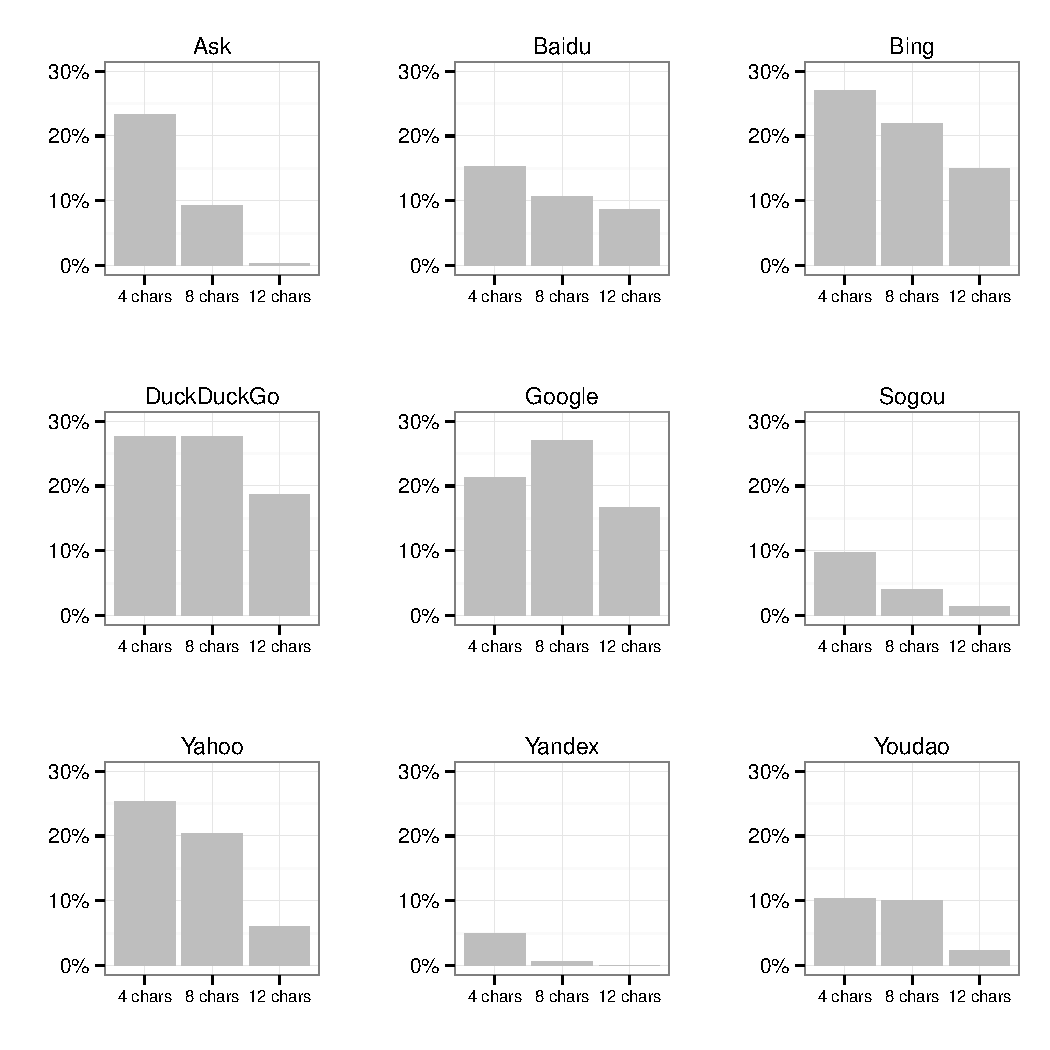
\includegraphics[width=\textwidth]{eng_vs_acc_9_way}}
  \caption{Accuracies for each length of each search engine compared}\label{fig:9searchengines}
\end{figure}

\end{document}
